\FloatBarrier
\section{Further results on the endogenous design}\label{app:escResults}\setcounter{equation}{0}
This appendix collects further results on the endogenous design of section \ref{sec:esc}: the UK and France, calibrated in full, under the cost calibrated on the U.S., and the path of the design along the projected U.S.\ demography.

\subsection{The UK and France}\label{app:escResults:countries}
For two of the 26 countries of section \ref{sec:esc:crossSection}, the UK and France, we have the household data to calibrate the model as fully as the U.S\@. Each is calibrated at $\rho = 1$ to its own pension spending, demography and design and with its own propensities to vote, the UK's households grouped at its own income cuts and France's at the U.S.\ income percentiles (appendix \ref{app:US}, table \ref{table:US:Calib}). This deep test takes the cost from the U.S.\ in two forms: the U.S.\ $\varepsilon = 20.44$, which gives each economy $n$ the parameter $\lambda_{n,t} = \varepsilon\,\Pi_{n,t}/R_{n,t}$ at its own ratio, and the U.S.\ $\lambda = 11.34$ (table \ref{table:US_ESC:calibration}), which at the U.S.\ ratio of 2020 is the same cost. Both are calibrated on the U.S.\ at its own household data, the CPS groups; the cross-section measures the U.S.\ from the OECD data, at which $\varepsilon = 20.01$ (appendix \ref{app:oecd26:anchor}). We read the test under $\varepsilon$, the transport of the cross-section, with $\lambda$ beside.

Table \ref{table:US_ESC:country} reports the designs the two electorates choose for 2020. Under $\varepsilon$ the UK, observed at $0.560$, chooses $0.673$, and France, observed at the Bismarckian corner, chooses $0.743$; under $\lambda$ they choose $0.690$ and $0.795$. Either way the three designs are ordered as observed, with the U.S.\ at $0.728$ between them. Under $\varepsilon$ the U.S.\ parameter accounts for a third of the distance from the U.S.\ design to the UK's and for little of the distance to France's, against about a quarter of each under $\lambda$. Both countries have a lower ratio $\Pi/R$ in 2020 than the U.S., so the U.S.\ $\varepsilon$ charges them less than the U.S.\ $\lambda$ does, and both choose flatter designs under it, which brings the UK closer to its observed design and takes France further from its own. No value of either parameter makes France re-elect its corner (appendix \ref{app:esc:cost}).

%% GENERATED by python/paper/build.py from results/ -- do not edit by hand.
%% Rebuild:  .venv\Scripts\python.exe python\paper\build.py --only US_ESC_Country
%% Source:   results/esc/escCountry.csv
\begin{table}[!htb]
\centering
\begin{threeparttable}
\caption{The UK and France under the U.S.\ cost of redistribution}
\label{table:US_ESC:country}
\renewcommand{\arraystretch}{1.25}
\begin{tabularx}{\textwidth}{lYYYYY}
\toprule
\textbf{Economy} & $\theta^{\ast}$ \textbf{observed} & \textbf{Tax rate} & $\theta$ \textbf{chosen, U.S.} $\lambda$ & \textbf{Own} $\lambda$ & $\tilde V$ \\
\midrule 
UK & 0.560 & 11.9\% & 0.625 & 7.264 & 0.223 \\ % row: gbr
France & 1.000 & 21.3\% & 0.749 & -- & 0.218 \\ % row: fra
UK at U.S.\ income groups & 0.543 & 11.9\% & 0.644 & 6.519 & 0.065 \\ % row: ukus
\bottomrule
\end{tabularx}
\begin{tablenotes}[flushleft]
\footnotesize
\item[] \textit{Note:} The cost is that of equation \eqref{eq:esc:budget}; $\lambda = 8.643$ is the U.S.\ value at $\rho = 1$, at which the U.S.\ electorate re-elects its observed design (section \ref{sec:esc:calibration}). Each economy is its own calibration at $\rho = 1$ ($\beta$ imposed from the U.S., $\omega$ its own; table \ref{table:US:Calib}); the UK at U.S.\ income groups is the UK workbook regrouped at the U.S.\ income percentiles. ``Chosen'' is the design in 2020 on the economy\textquotesingle s own freely simulated path under the U.S.\ parameter, to be read against the observed one; ``own'' is the value at which that path re-elects the observed design, with $\omega$ recalibrated at each trial value. No finite $\lambda$ makes France re-elect its observed design: it is the corner $\theta = 1$, and under a cost quadratic in the redistribution performed the first unit of redistribution is free at the margin.
\end{tablenotes}
\end{threeparttable}
\end{table}


The UK's own parameter, which re-elects its observed design, is $7.74$ as $\lambda$, a third below the U.S.\ value, and $14.66$ as $\varepsilon$, a little more than a quarter below. Table \ref{table:UK_ESC:calibration} calibrates $\lambda$ on the UK at each intertemporal elasticity as table \ref{table:US_ESC:calibration} does on the U.S\@. The UK's parameter lies below the U.S.\ one at low elasticities, by $33\%$ at $\rho = 0.5$ and $32\%$ at $\rho = 1$, and above it at $\rho = 2$, by $17\%$. The cost weighs less in the UK. At $\rho = 1$ its observed design loses $1.9\%$ of revenue, as the U.S.\ one does, but a flat benefit of the same size would lose $9.2\%$, against $22.9\%$ in the U.S., because the UK's dispersion of relative incomes is about half the U.S.\ one, $0.223$ against $0.436$, and its cost parameter a third lower, although its system is slightly larger, with a tax rate of $11.2\%$ against $10.5\%$. As in the U.S., the cost raises the calibrated political weight of the old, from $1.10$ to $1.15$ at $\rho = 1$.

%% GENERATED by python/paper/build.py from results/ -- do not edit by hand.
%% Rebuild:  .venv\Scripts\python.exe python\paper\build.py --only UK_ESC_Calibration
%% Source:   results/esc/escCountry.csv, escCalibrationCRRAUK.csv
\begin{table}[!htb]
\centering
\begin{threeparttable}
\caption{The calibrated cost of redistribution in the UK}
\label{table:UK_ESC:calibration}
\renewcommand{\arraystretch}{1.25}
\begin{tabularx}{.8\textwidth}{YYYYY}
\toprule
$\rho$ & $\lambda$ & $\omega$ & $1 - f(\theta^{\ast})$ & $1 - f(0)$ \\
\midrule 
0.5 & 15.117 & 1.76 & 3.8\% & 18.1\% \\ % row: rho@0.5
1.0 & 7.264 & 1.21 & 1.8\% & 9.2\% \\ % row: rho@1.0
2.0 & 2.777 & 1.06 & 0.7\% & 3.6\% \\ % row: rho@2.0
\bottomrule
\end{tabularx}
\begin{tablenotes}[flushleft]
\footnotesize
\item[] \textit{Note:} As table \ref{table:US_ESC:calibration}, for the UK at its own income groups, where $\theta^{\ast} = 0.560$ and $\tilde V = 0.223$ at every $\rho$; $\lambda$ is the value at which the UK electorate re-elects its observed design. $\beta$ is the U.S.\ value of the calibration without the cost, imposed as in section \ref{sec:oecd}, and $\omega$ is recalibrated with $\lambda$.
\end{tablenotes}
\end{threeparttable}
\end{table}


The cross-section of section \ref{sec:esc:crossSection} measures the UK differently, from the OECD earnings data at the U.S.\ income percentiles and with the U.S.\ propensities to vote. With its political weight of the old calibrated to its spending, in the second layer of the test, the UK chooses $0.791$ under the U.S.\ $\varepsilon$, above the U.S.\ design of $0.735$ at those data, where the deep test places it below the U.S.\ one (table \ref{table:OECD26:reconcile}). At its own propensities to vote, which rise less with income than the U.S.\ ones, the cross-section places it below the U.S.\ as well (\oa{esc-oecd26-turnout}), and under $\lambda$ the two tests place it on the same sides as under $\varepsilon$, at $0.690$ and $0.805$. For the UK the propensities to vote thus decide on which side of the U.S.\ design its predicted design falls, and the transport of the cost does not. Appendix \ref{app:oecd26} compares the two measurements of the three economies.

\FloatBarrier
\subsection{The design along the baseline path}\label{app:escResults:path}
Figure \ref{fig:US_ESC:path} follows the U.S.\ along its projected demography at $\rho = 1$, with the design chosen and with the design pinned at $\theta^{\ast}$. Since the calibration targets only the design of 2020, the path after 2020 is a prediction. Along it the chosen design goes from $0.728$ in 2020 to $0.802$ in 2050 and stays at $0.820$ from 2110 on. It tracks the number of workers per retiree, which falls from $1.34$ to $1.07$, and settles one period after the demography does. The tax rate climbs from $10.5\%$ to $16.9\%$, $0.3$ p.p.\ above the path with the design pinned, since a more earnings-related system loses less of its revenue.\footnote{The path barely depends on the Frisch elasticity. Recalibrated at $\xi = 0.2$ and $0.4$, $\lambda$ changes by less than one percent and the tax rate in 2110 by about $0.3$ p.p., while the design in 2110 and the design under acute ageing move by about $0.001$ (\oa{esc-parameters}).}

\begin{figure}[!htb]
    \centering
    \caption{The design and the tax along the baseline path}
    \label{fig:US_ESC:path}
\begin{threeparttable}
    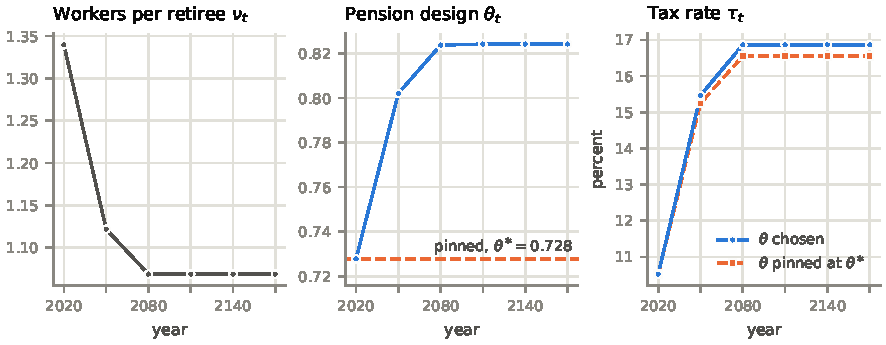
\includegraphics[width=\linewidth]{Figs/US_ESC_Path.pdf}\par
\begin{tablenotes}[flushleft]\footnotesize
    \item[]\textit{Note:} The paths start in 2020, the calibration year, under log preferences ($\rho = 1$); a design chosen at one date applies from the following one. The \oa{esc-paths} shows the paths from 1990 and for the UK and France, and its page \oanum{esc-paths-parameters} shows them at the other elasticities.
\end{tablenotes}
\end{threeparttable}
\end{figure}
